\documentclass[11pt]{article}
\usepackage{fullpage}
\usepackage{amsmath}
\usepackage{amssymb}
\usepackage{graphicx}
\usepackage{color}
\usepackage{float}
\usepackage{caption}
\usepackage{placeins}

\renewcommand\baselinestretch{1.5}
\newcommand{\reals}{\mathbb{R}}
\newcommand{\Pose}{{\cal P}}
\newcommand{\A}{{\cal A}} 
\newcommand{\X}{\mathbf{X}} 
\newcommand{\symb}{\Sigma}
\newcommand{\actP}{P^{\A}}
\newcommand{\B}{\cal B}
\newcommand{\Xrm}{\X^{\Am}_{-r}}
\newcommand{\Am}{\A_{m}} 
\begin{document}

\title{Jeroen's model}
\maketitle

\section{Notation}

\begin{itemize}

\item $\symb$: partially-ordered list of symbols (types).

\item $\symb_i$: ith symbol in partial ordering.

\item $T$: number of symbols in grammar.

\item $\Pose$: pose space.

\item $\Pose(b)$: pose cell of brick $b$- a set of poses. $\Pose(b) \in \Pose$ 

\item ${\B} = (b_1,\ldots,b_N)$: set of bricks.

\item $\A = (a_1,\ldots,a_M)$, $\A \subseteq {\B}$: set of active bricks.

\item $\Am = (a_1,\ldots,a_m)$, $m \leq M$ $\Am \subseteq {\A}$: subset of active bricks.

\item $t(b)$: type of brick $b$.

\item ${\cal R}$: set of production rules of the form
$A \rightarrow B_1,\ldots,B_k$ with $r = A,B_1,\ldots,B_k \in \Sigma$. ${\cal R}$ is acyclic.

\item $n(r)$: number of slots/children associated with rule $r \in {\cal R}$

%%%\item $c(b) = {\displaystyle \max_{r \in {\cal R}, LHS(r) = t(b)}} n(r): $ maximum number of slots/children associated with a brick $b$

\item $p_{r,n}(x_i|x)$, $r \in {\cal R}$, $x,x_i \in {\cal P}$, $n \in [1...n(r)]$: 
conditional probability density over pose for $B_i$ given pose for $A$ for this rule and slot.

\item ${\cal R}(A)$: rules with $A$ in the left-hand-side (LHS).

\item $p_A$: distribution over ${\cal R}(A)$.

\item $s_b \in \{0,1\}$: on/off state of brick $b$.

\item $r_b \in {\cal R}(t(b))$: rule used by brick $b$.

\item $\mathbf{g_b} \in ( {\B} \cup \perp )^{c(b)}$: array of pointers, where each element can either point to a brick, or null (no child).

\item $V(b)$: ``before'' set of bricks, which we define as $V(b) = \{b' : t(b') < t(b) \}$ where $<$ means ``comes before in the partial ordering defined by $\symb$''.

\item $W(b)$: ``after'' set of bricks, which we define as $V(b) = \{b' : t(b') > t(b) \}$ where $>$ means ``comes after in the partial ordering defined by $\symb$''.

\item $q_b \in \Pose(b)$: pose for brick $b$. $q_b = \perp$ is a special ``nothing'' pose that does not contribute to image evidence.

\item $\X = \{ \mathbf{s}, \mathbf{r}, \mathbf{g}, \mathbf{q}\}$: collection of hidden variables of model.

\item $\Xrm = \{s_a, g_a, q_a\}, \forall a \in \Am$: collection of hidden variables of model, with rules removed, for the set of bricks in the active set.

\item $I$: the image.

\end{itemize}

\section{Model}

\begin{figure}[htbp]
\begin{center}
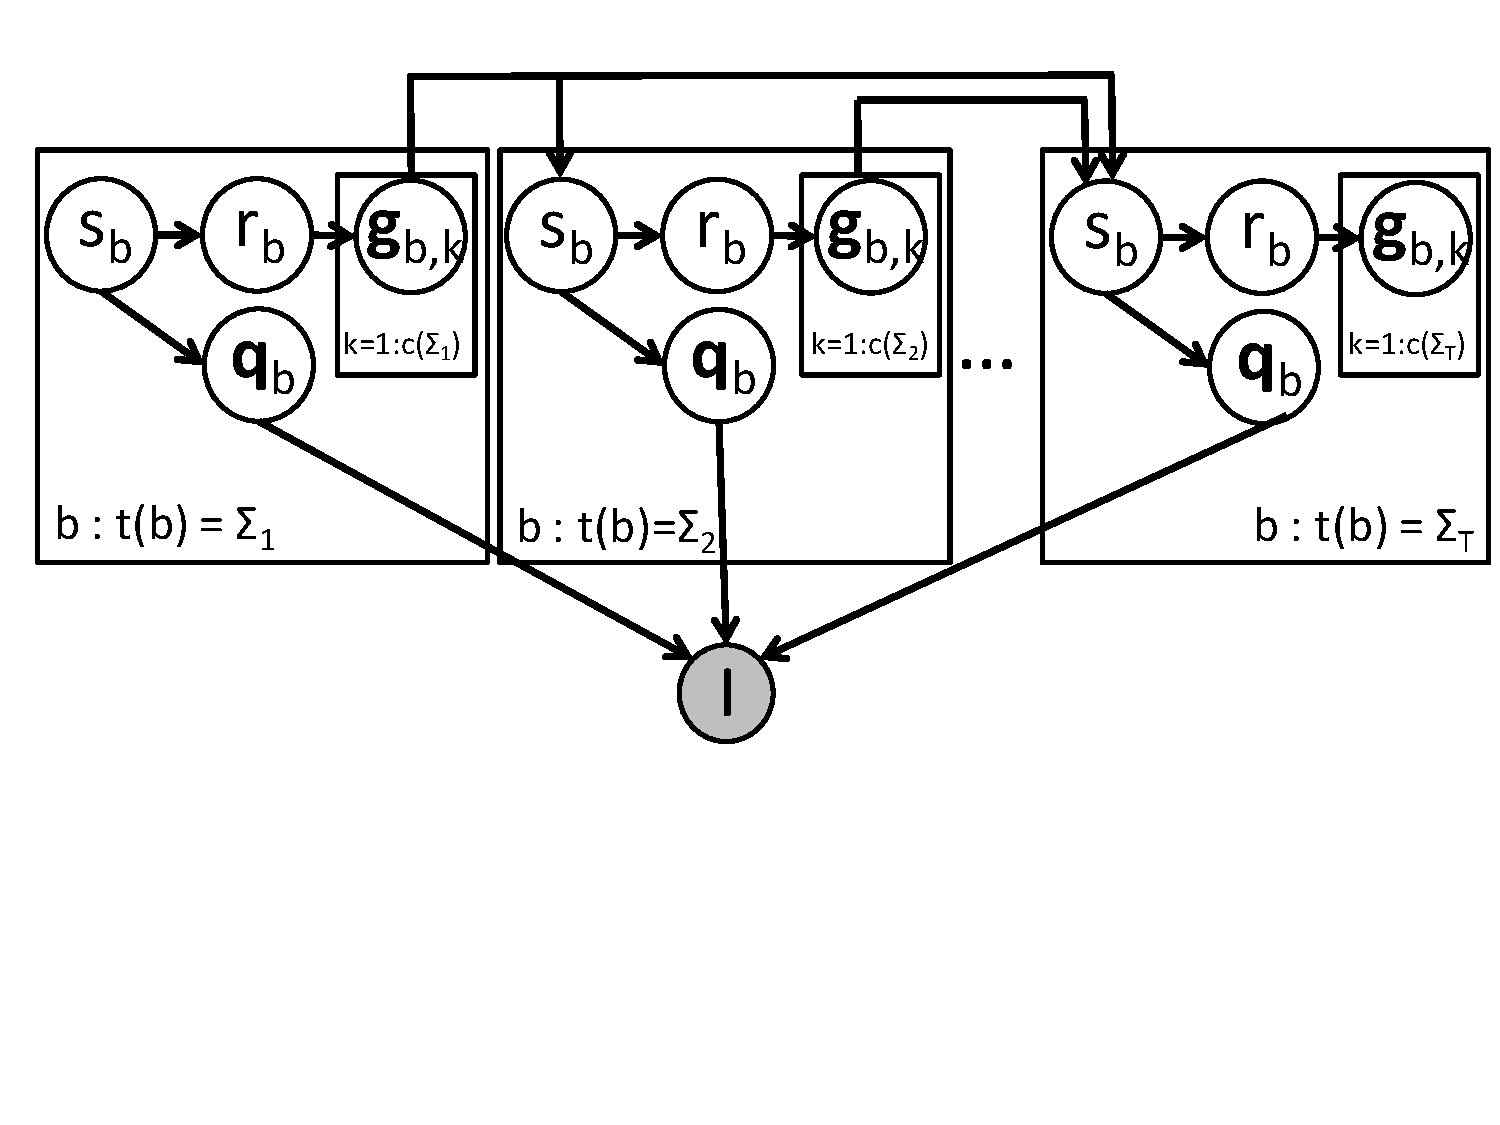
\includegraphics[width=\textwidth, trim=0cm 6cm 0cm 0cm]{gm.pdf}
\caption{Graphical model}
\end{center}
\end{figure}

\FloatBarrier

Joint probability is given by: \\

\begin{eqnarray}
P(\X, I) &=& \big({\displaystyle \prod_{b \in {\B}}} P(s_b \mid \mathbf{g}_{V(b)}) \big ) \\
& &\big( {\displaystyle \prod_{b \in {\B}}} P(r_b \mid s_b) {\displaystyle \prod_{k=1}^{c(b)}} P(g_{b,k} \mid r_b) \big) \\
& &\big( {\displaystyle \prod_{b \in {\B}}} P(\mathbf{q_b} \mid s_b)\big) \\
& & P(I \mid \mathbf{q})
\end{eqnarray}

Before we define localizations, we first define additional notation to ease the presentation.

\begin{itemize}
\item $\mathbf{g}_b^{\Am} \in ( {\Am} \cup \emptyset )^{c(b)}$: array of pointers, where each element can either point to a brick in the active set defined by $\Am$, or blank (child not yet specified) denoted by $\emptyset$. Note that blank is \textbf{different} than null (no child) in that blank means ``there could be a child in this slot, but we don't know if there is or which one yet'' while null (no child) means ``there definitely isn't a child in this slot''.
\end{itemize}

\section*{Localization}

%For localization, we do not explicitly represent $\mathbf{r}$; instead we express the state configuration in terms of $\mathbf{g}_b^{\A}$ only, which implicitly specifies a set of compatible rules. Rather than selecting specific values for $\mathbf{r}$, we instead marginalize over the set of compatible rules defined by $\mathbf{g^{\A}}$ wherever  $\mathbf{r}$ is referred to.

We define localizations in terms of the components $\big({\displaystyle \prod_{b \in {\B}}} P(s_b \mid \mathbf{g}_{V(b)}) \big )$, $\big( {\displaystyle \prod_{b \in {\B}}} P(r_b \mid s_b) {\displaystyle \prod_{k=1}^{c(b)}} P(g_{b,k} \mid r_b) \big)$, $\big( {\displaystyle \prod_{b \in {\B}}} P(\mathbf{q_b} \mid s_b)\big)$, and $P(I \mid \mathbf{q})$ separately.

\begin{eqnarray}
\big({\displaystyle \prod_{b \in {\B}}} P(s_b \mid \mathbf{g}_{V(b)}) \big ) &\Rightarrow& \big({\displaystyle \prod_{a \in {\Am}}} P(s_a \mid \mathbf{g}^{\Am}_{V({b})}) \big )
\end{eqnarray}

where $\Rightarrow$ is used to mean ``localiizes to''. Similarily, 

\begin{eqnarray}
\big( {\displaystyle \prod_{b \in {\B}}} P(r_b \mid s_b) {\displaystyle \prod_{k=1}^{c(b)}} P(g_{b,k} \mid r_b) \big) &\Rightarrow& \big( {\displaystyle \prod_{a \in \Am}} P(r_a \mid s_a) {\displaystyle \prod_{k=1}^{c(b)}} P^{\Am}(g_{a,k} \mid r_a) \big) \\
%
P^{\Am}(g_{a,k} \mid r_a) &=& \begin{cases} \label{actPg} 1-{\displaystyle \sum_{a' \in {\Am}}} P(g_{a,k} = a' \mid r_a) \mbox{ if } g_{a,k} == \emptyset \\
 P(g_{a,k} \mid r_a) \mbox{ , otherwise } \end{cases}
\end{eqnarray}
Note that the RHS of Eqn. (\ref{actPg}) is defined in terms of non-localized distributions, $P(g_{a,k} \mid r_a)$.

\begin{eqnarray}
\big( {\displaystyle \prod_{b \in {\B}}} P(\mathbf{q_b} \mid s_b)\big) \Rightarrow \big( {\displaystyle \prod_{a \in {\Am}}} P(\mathbf{q_a} \mid s_a)\big)
\end{eqnarray}
\begin{eqnarray}
P(I \mid \mathbf{q}) \Rightarrow P(I \mid \mathbf{q^{\Am}})
\end{eqnarray}

We define the overall localized distribution, $P^{\Am}(X^{\Am}$, I), in terms of the previously defined localization distributions:
\begin{eqnarray}
P^{\Am}(X^{\Am}, I)
&=& \big({\displaystyle \prod_{a \in {\Am}}} P(s_a \mid \mathbf{g}^{\Am}_{V({b})}) \big ) \\
& & \big( {\displaystyle \prod_{a \in {\Am}}} P(r_a \mid s_a) {\displaystyle \prod_{k=1}^{c(b)}} P^{\Am}(g_{a,k} \mid r_a) \big) \\
& & {\displaystyle \prod_{a \in {\Am}}} P(\mathbf{q_a} \mid s_a)\big) \\
& & P(I \mid \mathbf{q^{\Am}})
\end{eqnarray}

\section*{State representation}

Representing the configuration of an image for a \textbf{non-localized} model requires specifying $s_b$, $g_b$, $r_b$, $q_b$, $\forall b \in \B$. For a \textbf{localized} model, the same random variables could be used as the state representation. However, requiring specification of $r_b$ is too restrictive; we may not be able to well predict the rule a brick has used by examining the set of active bricks. This is especially true if the active set only contains one brick! Instead, we represent the state representation of the localized model by the random variables $\Xrm = \{s_a$, $g_a$, $q_a\}$, $\forall a \in \A$, and we marginalize over $r_a$ wherever it is used.

\section*{Inference}

Inference proceeds by iteratively adding one brick at a time to the active set. At any iteration, $m$, our goal is to maintain a representation of the localized posterior distribution $P^{\Am}(\Xrm \mid I)$. To maintain this representation, we employ a particle filtering approach. We treat samples from the previous localized posterior distribution $P^{\A_{m-1}}(\X^{\A_{m-1}}_{-r} \mid I)$ as draws from a proposal distribution, and re-weight these particles according to

%\begin{figure}[htbp]
%\begin{center}
%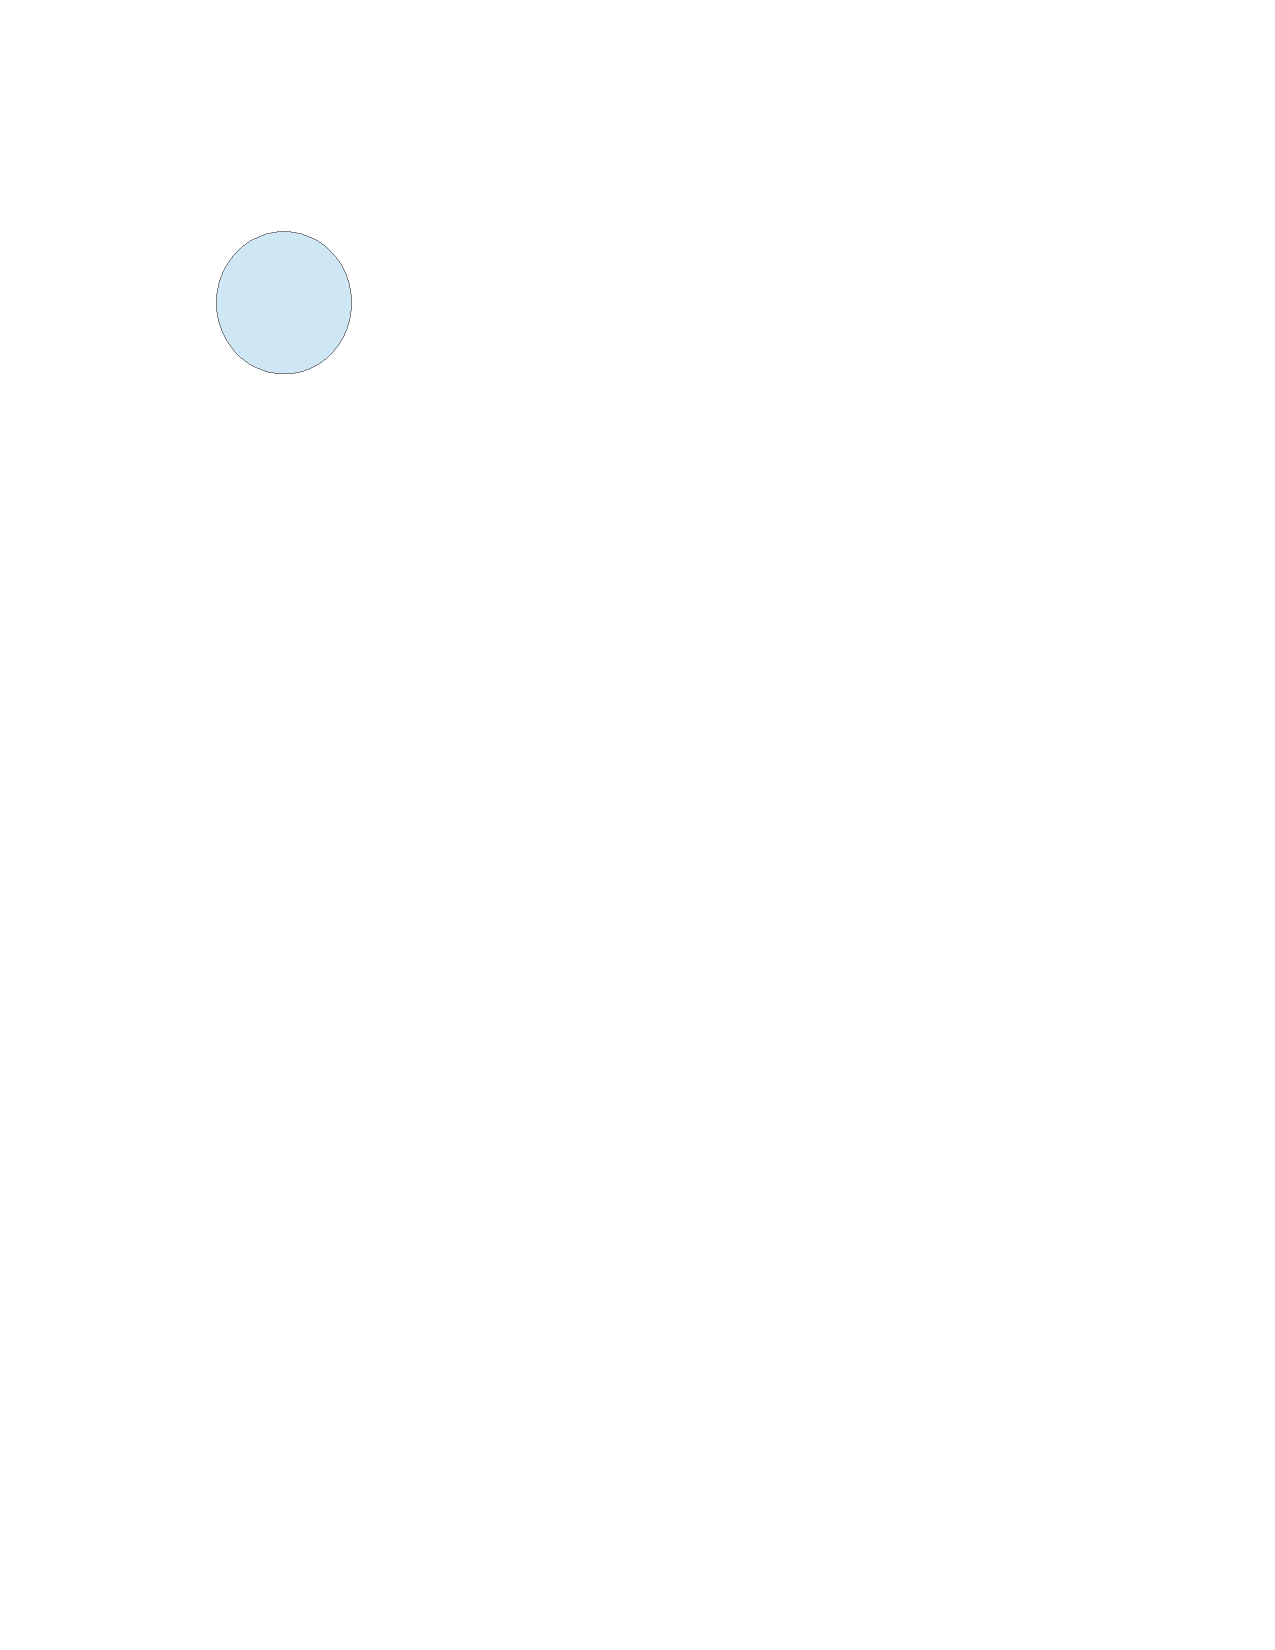
\includegraphics[width=\textwidth]{test.pdf}
%\caption{Graphical model}
%\end{center}
%\end{figure}


\end{document}
